

\usetikzlibrary{calc}

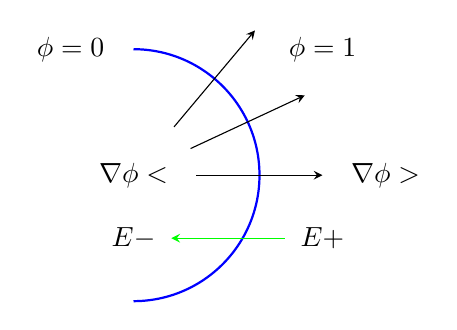
\begin{tikzpicture}[x={(0.8cm,0cm)}, y={(0cm,0.8cm)}, z={(-3.85mm, -3.85mm)}]
\def\rayon{3}
%styledesnœuds
\tikzstyle{textLine}=[rectangle, text=black]
\tikzstyle{textw}=[rectangle, text=black]
\tikzstyle{pointx}=[circle, fill, scale=0.2]
\tikzstyle{vector}=[-stealth,thin]



%curved interface
\coordinate (c0) at (1,0);
\coordinate (c1) at (-90:2);
\coordinate (c2) at (90:2);
\coordinate (mid) at ($(c1)!0.5!(c2)$);
\draw[thick,blue] ++(c1) arc (-90:90:2);

%normal vectors
\draw[vector] ($(mid)+(0:1)$) -- ($(mid)+(0:3)$);
\draw[vector] ($(mid)+(25:1)$) -- ($(mid)+(25:3)$);
\draw[vector] ($(mid)+(50:1)$) -- ($(mid)+(50:3)$);

%texts
\node[textLine, text centered] (chg) at ($(c2)-(1,0)$) { $\phi=0$};
\node[textLine, text centered] (chg) at ($(c2)+(3,0)$) { $\phi=1$};
\node[textLine, text centered] (chg) at ($(mid)$) { $\nabla\phi<$};
\node[textLine, text centered] (chg) at ($(mid)+(0:4)$) { $\nabla\phi>$};
\node[textLine, text centered] (em) at ($(mid)-(0,1)$) { $E-$};
\node[textLine, text centered] (ep) at ($(mid)+(0:3)-(0,1)$) { $E+$};

\draw[vector, color=green] ($(ep)!0.2!(em)$) -- ($(ep)!0.8!(em)$);
\end{tikzpicture}
